%!TEX root = ../../book_ML.tex
\chapter{Thuật toán học perceptron}
\label{cha:pla}
% Cứ làm đi, sai đâu sửa đấy, cuối cùng sẽ thành công!

% Đó chính là ý tưởng chính của một thuật toán rất quan trọng trong Machine Learning - thuật toán Perceptron Learning Algorithm hay PLA.




\section{Giới thiệu}
\index{thuật toán học perceptron -- perceptron learning algorithm}
\index{perceptron learning algorithm -- thuật toán học perceptron}
\index{PLA}
\index{phân loại nhị phân -- binary classification}
\index{binary classification -- phân loại nhị phân}
Trong chương này, chúng ta cùng tìm hiểu một trong các thuật toán xuất hiện đầu
tiên trong lịch sử machine learning. Đây là một phương pháp phân loại đơn giản
có tên là \textit{thuật toán học perceptron} ({perceptron learning
algorithm} -- PLA~\cite{rosemblat1957perceptron}). Thuật toán này được thiết kế
cho bài toán \textit{phân loại nhị phân} khi dữ liệu chỉ thuộc một trong hai
nhãn. Đây là nền tảng cho các thuật toán liên quan tới mạng neuron nhân tạo và
gần đây là deep learning.

% Xét một bài toán phân loại đơn giản với chỉ cho trường hợp đơn giản nhất: chỉ có hai class (lớp) (\textit{bài toán với chỉ hai class được gọi là binary classification}) và cũng chỉ hoạt động được trong một trường hợp rất cụ thể. Tuy nhiên, nó là nền tảng cho một mảng lớn quan trọng của Machine Learning là Neural Networks và sau này là Deep Learning. (Tại sao lại gọi là Neural Networks - tức mạng dây thần kinh - các bạn sẽ được thấy ở cuối bài).



Giả sử có hai tập dữ liệu hình vuông và tròn như được minh hoạ trong
Hình~\ref{fig:9_1a}. Bài toán đặt ra là từ dữ liệu của hai tập được gán nhãn cho
trước, hãy xây dựng một bộ phân loại có khả năng dự đoán nhãn của một điểm
dữ liệu mới, chẳng hạn điểm hình tam giác màu xám.

\index{class boundary}
\index{siêu phẳng -- hyperplane}
\index{hyperplane -- siêu phẳng}

Nếu coi mỗi vector đặc trưng là một điểm trong không gian nhiều chiều, bài toán
phân loại có thể được coi như bài toán xác định nhãn của từng điểm trong không
gian. Nếu coi mỗi nhãn {chiếm} một hoặc vài vùng trong không gian, ta cần đi tìm
{ranh giới} giữa các vùng đó. Ranh giới đơn giản nhất trong không gian hai chiều
là một đường thẳng, trong không gian ba chiều là một mặt phẳng, trong không gian
nhiều chiều là một \textit{siêu phẳng}. Những ranh giới phẳng này đơn giản vì
chúng có thể được biểu diễn bởi một hàm số tuyến tính. Hình~\ref{fig:9_1b} minh
họa một đường thẳng phân chia hai tập dữ liệu trong không gian hai chiều. Trong
trường hợp này, điểm dữ liệu mới hình tam giác rơi vào cùng tập hợp với các điểm
hình tròn.

\index{tách biệt tuyến tính -- linearly separable}
\index{linearly separable -- tách biệt tuyến tính}
PLA là một thuật toán đơn giản giúp tìm ranh giới siêu phẳng cho bài toán phân loại nhị phân trong trường hợp tồn tại siêu phẳng đó. Nếu hai tập dữ liệu có thể được phân chia hoàn toàn bằng một siêu phẳng, ta nói rằng hai tập đó \textit{tách biệt tuyến tính} ({linearly separable}).

% Ranh giới này được xác định dựa trên dữ liệu huấn luyện.

% Hiểu theo một cách khác, chúng ta cần tìm \textit{lãnh thổ} của mỗi class sao cho, với mỗi một điểm mới, ta chỉ cần xác định xem nó nằm vào lãnh thổ của class nào rồi quyết định nó thuộc class đó. Để tìm \textit{lãnh thổ} của mỗi class, chúng ta cần đi tìm biên giới (boundary) giữa hai \textit{lãnh thổ} này. Vậy bài toán classification có thể coi là bài toán đi tìm boundary giữa các class.

\begin{figure}[t]
\begin{subfigure}{0.49\textwidth}
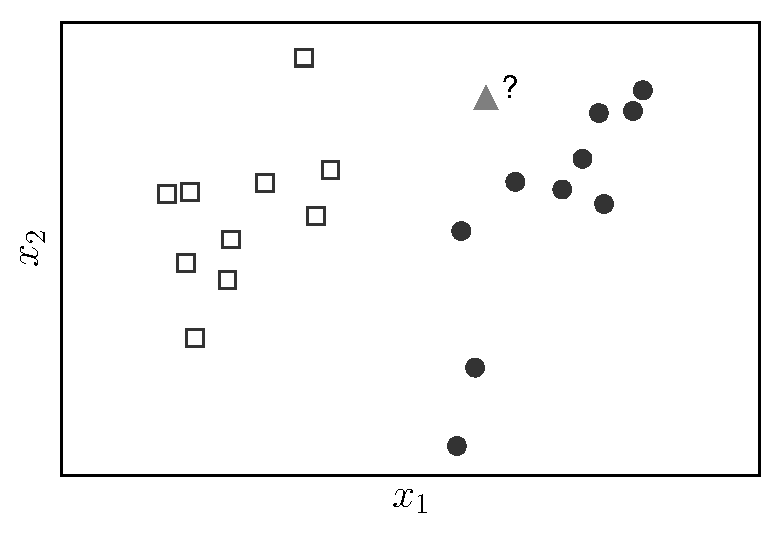
\includegraphics[width=0.99\linewidth]{ebookML_src/src/perceptron/pla1.pdf}
\caption{}
\label{fig:9_1a}
\end{subfigure}
\begin{subfigure}{0.49\textwidth}
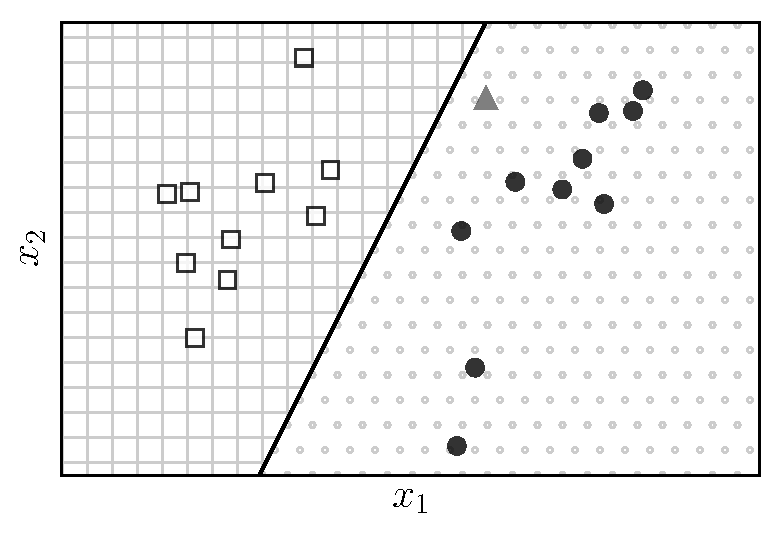
\includegraphics[width=0.99\linewidth]{ebookML_src/src/perceptron/pla2.pdf}
\caption{}
\label{fig:9_1b}
\end{subfigure}
\caption{
Bài toán phân loại nhị phân trong không gian hai chiều. (a) Cho hai tập dữ liệu được gán nhãn vuông và tròn, hãy xác định nhãn của điểm tam giác. (b) Ví dụ về một ranh giới phẳng phân chia hai tập hợp. Điểm tam giác được phân vào tập các điểm hình tròn.
}
\label{fig:9_1}
\end{figure}







% \textbf{Bài toán Perceptron }

% Bài toán Perceptron được phát biểu như sau. \textit{Cho hai lớp dữ liệu linearly separable, hãy tìm một siêu phẳng sao cho toàn bộ các điểm thuộc một lớp nằm về một phía của siêu phẳng đó, và khác phía với mọi điểm thuộc lớp còn lại.}




% Nếu tồn tại một đường phẳng phân chia hai class thì ta gọi hai class đó là \textit{linearly separable}. Các thuật toán classification tạo ra các boundary là các đường phẳng được gọi chung là Linear Classifier.


\section{Thuật toán học perceptron}
% Cũng giống như các thuật toán lặp trong \href{http://machinelearningcoban.com/2017/01/01/kmeans/}{K-means Clustering} và \href{http://machinelearningcoban.com/2017/01/12/gradientdescent/}{Gradient Descent}, ý tưởng cơ bản của PLA là xuất phát từ một nghiệm dự đoán nào đó, qua mỗi vòng lặp, nghiệm sẽ được cập nhật tới một ví trí tốt hơn. Việc cập nhật này dựa trên việc giảm giá trị của một hàm mất mát nào đó.

% Chúng ta cùng đi xây dựng một hàm mất mát và đi tìm nghiệm tối ưu cho hàm mất mát đó.


\subsection{Quy tắc phân loại}
Giả sử $\mathbf{X} = [\mathbf{x}_1, \mathbf{x}_2, \dots, \mathbf{x}_N] \in \mathbb{R}^{d \times N}$ là ma trận chứa tập huấn luyện mà mỗi cột $\mathbf{x}_i$ là một điểm dữ liệu trong không gian $d$ chiều.
Các nhãn được lưu trong một vector hàng $\mathbf{y} = [y_1, y_2, \dots, y_N] \in \mathbb{R}^{1\times N}$ với $y_i = 1$ nếu $\mathbf{x}_i$ mang nhãn vuông và $y_i = -1$ nếu $\mathbf{x}_i$ mang nhãn tròn.

Tại một thời điểm, giả sử ranh giới là một siêu phẳng có phương trình
\begin{eqnarray}
f_{\mathbf{w}}(\mathbf{x}) &=& w_1x_1 + \dots + w_dx_d + w_0 =\bx^T\bw + w_0 = 0
\end{eqnarray}
với $\bw \in \R^d$ là vector trọng số và $w_0$ là hệ số điều chỉnh. Bằng cách sử dụng thủ thuật gộp hệ số điều chỉnh (xem Mục~\ref{ssec:3_biastrick}), ta có thể coi phương trình siêu phẳng là
$f_{\bw}(\bx) = \bx^T\bw = 0$ với $\bx$ ở đây được ngầm hiểu như vector đặc
trưng mở rộng thêm một đặc trưng bằng một. Vector trọng số $\bw$ chính là
\textit{vector pháp tuyến} của siêu phẳng $\bx^T\bw = 0$.


% với $\mathbf{\bar{x}}$ là điểm dữ liệu mở rộng bằng cách thêm phần tử $x_0 = 1$ lên trước vector $\mathbf{x}$ tương tự như trong \href{http://machinelearningcoban.com/2016/12/28/linearregression/}{Linear Regression}. Và từ đây, khi nói $\mathbf{x}$, tôi cũng ngầm hiểu là điểm dữ liệu mở rộng.



% <div class="imgcap">
% <img src ="\assets\pla\pla4.png" align = "center" width = "400">
% <div class = "thecap">Hình 2: Phương trình đường thẳng boundary.</div>
% </div>
\begin{figure}[t]
\begin{subfigure}{0.49\textwidth}
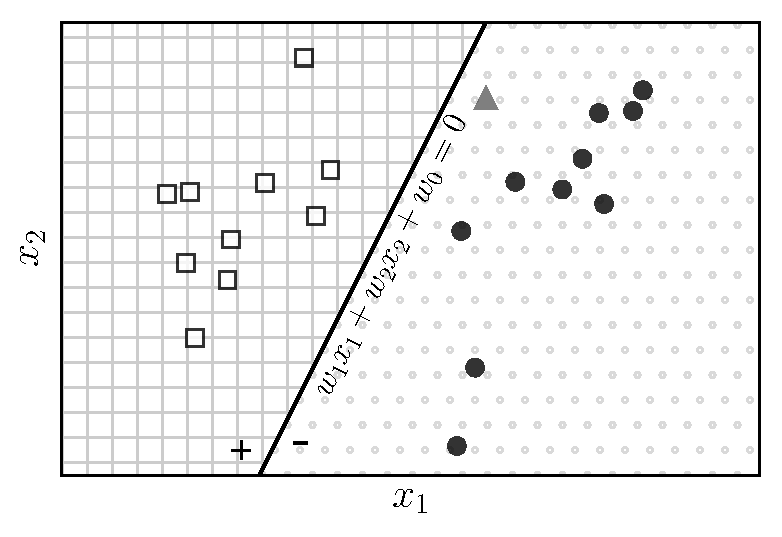
\includegraphics[width=0.99\linewidth]{ebookML_src/src/perceptron/pla4.pdf}
\caption{Đường thẳng phân chia không gây lỗi, mọi điểm được phân loại đúng.}
\label{fig:9_2a}
\end{subfigure}
\begin{subfigure}{0.49\textwidth}
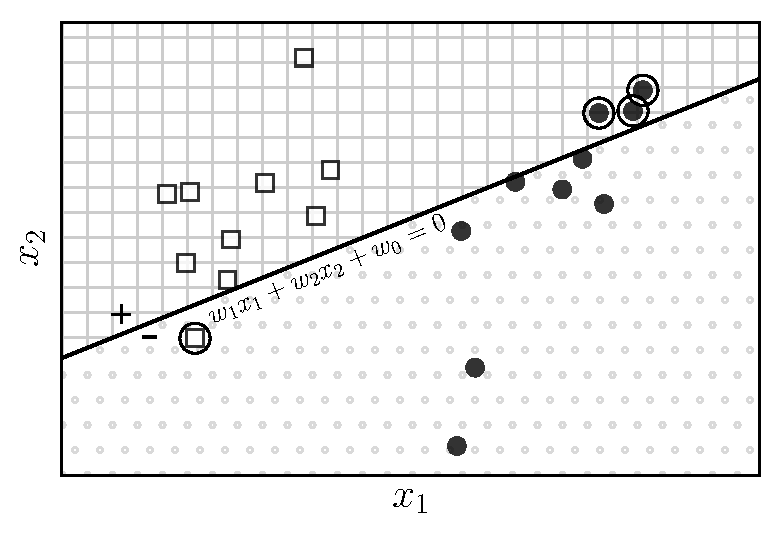
\includegraphics[width=0.99\linewidth]{ebookML_src/src/perceptron/pla3.pdf}
\caption{Đường thẳng phân chia gây ra lỗi tại các điểm được khoanh tròn.}
\label{fig:9_2b}
\end{subfigure}
\caption{
Ví dụ về các đường thẳng trong không gian hai chiều: (a) một nghiệm của bài toán PLA, (b) đường thẳng không phân chia chính xác hai lớp.
}
\label{fig:9_2}
\end{figure}

% \begin{figure}[t]
%     \begin{subfigure}{0.49\textwidth}
%     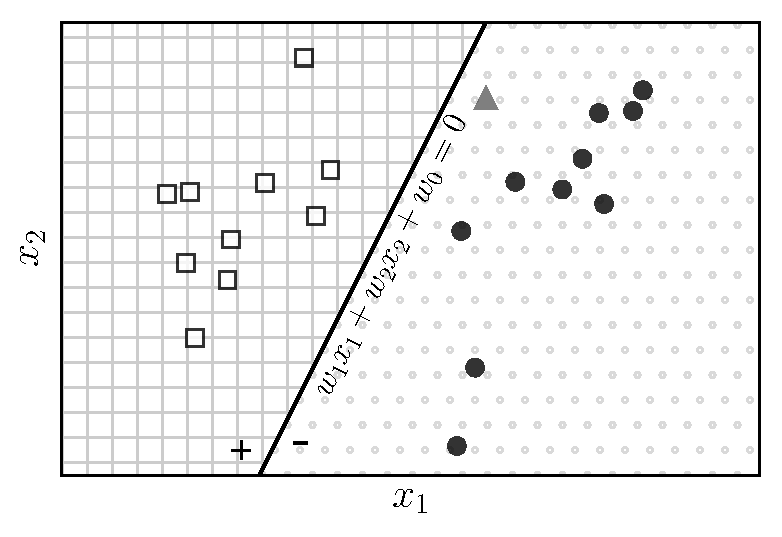
\includegraphics[width=0.99\linewidth]{ebookML_src/src/perceptron/pla4.pdf}
%     \caption{}
%     \label{fig:9_2a}
%     \end{subfigure}
%     \begin{subfigure}{0.49\textwidth}
%     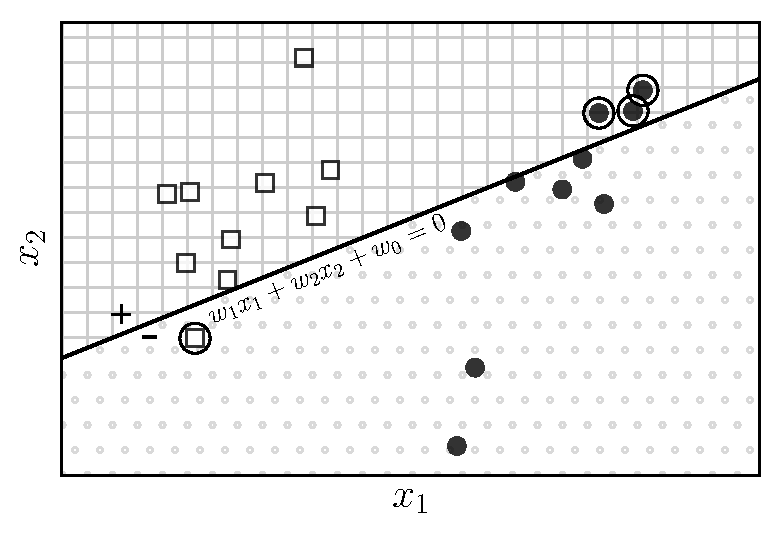
\includegraphics[width=0.99\linewidth]{ebookML_src/src/perceptron/pla3.pdf}
%     \caption{}
%     \label{fig:9_2b}
%     \end{subfigure}
%     \caption{

%     }
%     \label{fig:9_2}
% \end{figure}


% \begin{figure}[t]
%      % caption on side
%      \floatbox[{\capbeside\thisfloatsetup{capbesideposition={right,top},capbesidewidth=6cm}}]{figure}[\FBwidth]
%      {\caption{
%      Phương trình đường thẳng phân chia hai lớp.
%      }
%      \label{fig:9_2}}
%      { % figure here
%      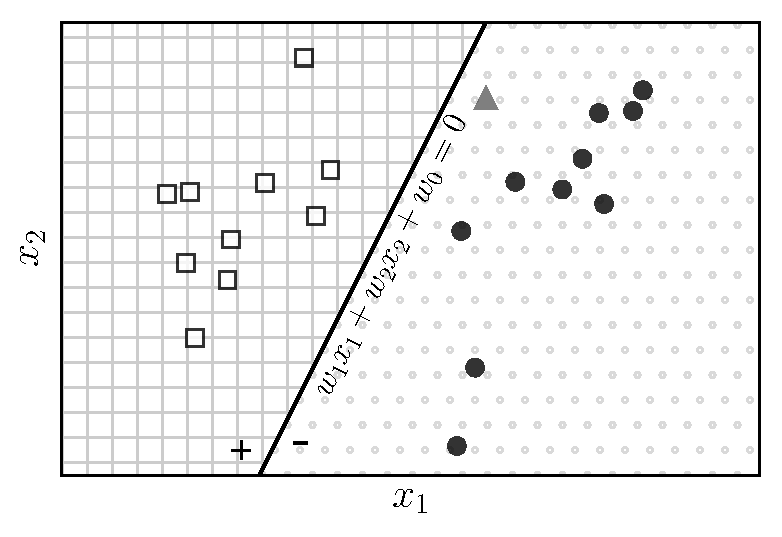
\includegraphics[width=.5\textwidth]{ebookML_src/src/perceptron/pla4.pdf}
%      }
%  \end{figure}

Trong không gian hai chiều, giả sử đường thẳng $w_1 x_1 + w_2 x_2 + w_0 = 0$ là
nghiệm cần tìm như Hình~\ref{fig:9_2a}. Ta thấy rằng các điểm nằm cùng phía so với đường thẳng này làm cho hàm số $f_{\mathbf{w}}(\mathbf{x})$ mang
cùng dấu. Nếu cần thiết, ta có thể đổi dấu của $\bw$ để các
điểm trên nửa mặt phẳng nền kẻ ô vuông mang dấu dương (+), các điểm trên nửa mặt phẳng nền chấm mang dấu âm (-). Các dấu này tương đương với
nhãn $y$ của mỗi điểm dữ liệu. Như vậy, nếu $\mathbf{w}$ là một nghiệm của bài toán thì nhãn của một điểm dữ liệu mới $\mathbf{x}$ được xác định bởi% \begin{equation}
% \text{label}(\mathbf{x}) = 1 ~\text{if}~ \mathbf{w}^T\mathbf{x} \geq 0, \text{otherwise} -1
% \end{equation}
\begin{align}
\label{eqn:9_sign}
\text{label}(\bx) = \left\{
\begin{matrix}
1 & \text{nếu}~ \bx^T\bw \geq 0\\
-1 & \text{trường hợp còn lại}
\end{matrix}
\right.
\end{align}
Vậy,
\begin{math}
\text{label}(\mathbf{x}) = \text{sgn}(\mathbf{w}^T\mathbf{x})
\end{math}
với $\text{sgn}$ là hàm xác định dấu. Quy ước $\text{sgn}(0) = 1$.


\subsection{Xây dựng hàm mất mát}
\index{phân loại lỗi -- misclassified}
\index{misclassified -- phân loại lỗi}
Tiếp theo, chúng ta xây dựng một hàm mất mát theo tham số $\mathbf{w}$ bất kỳ.
Vẫn trong không gian hai chiều, xét đường thẳng $w_1x_1 + w_2x_2 + w_0 = 0$ được
cho như Hình~\ref{fig:9_2b}. Các điểm khoanh tròn là các điểm bị \textit{phân
loại lỗi}. Tham số $\bw$ là một nghiệm của bài toán nếu nó không gây ra điểm bị phân loại lỗi nào. Như vậy, hàm đếm số lượng điểm bị phân loại lỗi có thể coi là hàm mất mát của mô hình. Ta sẽ tìm cách tối thiểu hàm số này.

Nếu một điểm $\bx_i$ với nhãn $y_i$ bị phân loại lỗi, ta có $\sgn(\bx^T\bw)
\neq y_i$. Vì hai giá trị này chỉ bằng $1$ hoặc $-1$, ta phải có
$y_i\sgn(\bx_i^T\bw) = -1$. Như vậy, hàm đếm số lượng điểm bị phân loại lỗi có
thể được viết dưới dạng
\begin{equation}
J_1(\mathbf{w}) = \sum_{\mathbf{x}_i \in \mathcal{M}} (-y_i\text{sgn}(\bx_i^T\bw))
\end{equation}
trong đó $\mathcal{M}$ ký hiệu tập các điểm bị phân loại lỗi ứng với mỗi $\bw$. Mục đích cuối cùng là đi tìm $\bw$ sao cho mọi điểm trong tập huấn luyện đều được phân loại đúng, tức $J_1(\bw) = 0$. Một điểm quan trọng cần lưu ý là hàm mất mát $J_1(\bw)$ rất khó được tối ưu vì $\sgn$ là một hàm rời rạc. Chúng ta cần tìm một hàm mất mát khác để việc tối ưu khả thi hơn.
Xét hàm
\begin{equation}
J(\mathbf{w}) = \sum_{\mathbf{x}_i \in \mathcal{M}} (-y_i\bx_i^T\bw).
\end{equation}
Trong hàm số này, hàm rời rạc $\text{sgn}$ đã được lược bỏ. Ngoài ra, khi một
điểm phân loại lỗi $\mathbf{x}_i$ nằm càng xa ranh giới, giá trị
$-y_i\bx_i^T\bw$ sẽ càng lớn, khiến cho hàm mất mát cũng càng lớn. Lưu ý rằng
hàm mất mát chỉ được tính trên các tập điểm bị phân loại lỗi $\mathcal{M}$, giá
trị nhỏ nhất của hàm số này cũng bằng không nếu $\mathcal{M}$ là một tập rỗng.
Vì vậy, $J(\bw)$ được cho là tốt hơn $J_1(\bw)$ vì nó \textit{trừng phạt rất
nặng những điểm lấn sâu sang lãnh thổ của tập còn lại}. Trong khi đó,
$J_1(\bw)$ \textit{trừng phạt} các điểm phân loại lỗi một lượng như nhau và đều
bằng một, bất kể chúng gần hay xa ranh giới.

\subsection{Tối ưu hàm mất mát}
Tại một thời điểm, nếu chỉ quan tâm tới các điểm bị phân loại lỗi thì hàm số
$J(\mathbf{w})$ khả vi tại mọi $\bw$. Vậy ta có thể sử dụng GD hoặc SGD để tối
ưu hàm mất mát này. Chúng ta sẽ giải quyết bài toán tối ưu hàm mất mát $J(\bw)$
bằng SGD. Nếu chỉ {một} điểm dữ liệu $\mathbf{x}_i$ bị phân loại lỗi, hàm mất
mát và gradient của nó lần lượt là
\begin{equation}
J(\mathbf{w}; \mathbf{x}_i; y_i) = -y_i\bx_i^T\bw; \quad
% \end{equation}
% Đạo hàm tương ứng:
% \begin{equation}
\nabla_{\mathbf{w}}J(\mathbf{w}; \mathbf{x}_i; y_i) = -y_i\mathbf{x}_i
\end{equation}
Quy tắc cập nhật $\bw$ sử dụng SGD là
\begin{equation}
\mathbf{w} \leftarrow \mathbf{w} - \eta (-y_i\mathbf{x}_i) = \bw + \eta y_i\bx_i
\end{equation}
với $\eta$ là tốc độ học. Trong PLA, $\eta$ được chọn bằng 1. Ta có một quy tắc cập nhật rất gọn:
\begin{equation}
\mathbf{w}_{t+1} = \mathbf{w}_{t} + y_i\mathbf{x}_i
\end{equation}
Tiếp theo, ta thấy rằng
\begin{equation}
\bx_i^T\bw_{t+1} = \bx_i^T(\bw_t + y_i\bx_i) \\\
= \bx_i^T\bw_t + y_i \|\mathbf{x}_i\|_2^2.
\end{equation}
Nếu $\bx_i$ bị phân loại lỗi và có nhãn đúng $y_i = 1$, ta có
$\mathbf{x}_{i}^T\mathbf{w}_t < 0$. Cũng vì $y_i = 1$ nên $y_i
\|\mathbf{x}_i\|_2^2 = \|\mathbf{x}_i\|_2^2 \geq 1$ (chú ý $\bx_i$ là một vector đặc
trưng {mở rộng} với một phần tử bằng một). Từ đó suy ra $\bx_i^T\bw_{t+1} > \bx_i^T\bw_t$. Nói cách khác,
$-y_i\bx_i^T\bw_{t+1} < -y_i\bx_i^T\bw_t$. Điều tương tự cũng xảy ra với $y_i = -1$.
Việc này chỉ ra rằng đường thẳng được mô tả bởi $\bw_{t+1}$ có xu hướng khiến
hàm mất mát tại điểm bị phân loại lỗi $\bx_i$ giảm đi. \textit{Chú ý rằng việc
này không đảm bảo hàm mất mát tổng cộng sẽ giảm, vì rất có thể siêu
thẳng mới sẽ làm cho một điểm lúc trước được phân loại đúng trở thành một điểm bị
phân loại lỗi. Tuy nhiên, thuật toán này được đảm bảo sẽ hội tụ sau một số hữu
hạn bước.} Thuật toán perceptron được tóm tắt dưới đây:


% \subsection{Tóm tắt PLA }
\begin{myalg}{Perceptron}{pla}
\begin{enumerate}
\item Tại thời điểm $t = 0$, chọn ngẫu nhiên một vector trọng số $\mathbf{w}_0$.

\item Tại thời điểm $t$, nếu không có điểm dữ liệu nào bị phân loại lỗi, dừng thuật toán.

\item Giả sử $\bx_i$ là một điểm bị phân loại lỗi, cập nhật
\begin{equation}
\nonumber
\mathbf{w}_{t+1} = \mathbf{w}_t + y_i\mathbf{x}_i
\end{equation}

\item Thay đổi $t = t + 1$ rồi quay lại Bước 2.
\end{enumerate}
\end{myalg}

% Quy tắc cập nhật ở thuật toán \ref{alg:pla} có thể được phát biểu bằng lời như sau. Bắt đầu bằng một siêu phẳng bất kỳ trong không gian. Nếu không có điểm nào bị phân loại lỗi thì dừng thuật toán. Nếu có, chọn một điểm bất kỳ bị phân loại lỗi, nhân điểm đó với nhãn của nó rồi cộng vào \textit{vector pháp tuyến} của siêu phẳng hiện tại.

\subsection{Chứng minh hội tụ}

Gọi $\mathbf{w}^*$ là một nghiệm của bài toán phân loại nhị phân. Nghiệm này luôn tồn tại khi hai tập dữ liệu tách biệt tuyến tính. Ta sẽ chứng minh bằng phản chứng Thuật toán~\ref{alg:pla} kết thúc sau một số hữu hạn bước.

Giả sử ngược lại, tồn tại một điểm xuất phát $\bw$ khiến Thuật
toán~\ref{alg:pla} chạy vô hạn bước. Trước hết ta thấy rằng, nếu $\mathbf{w}^*$ là nghiệm thì $\alpha\mathbf{w}^*$ cũng là nghiệm của
bài toán với $\alpha > 0$ bất kỳ. Xét dãy số không âm $ u_{\alpha}(t) = \|\mathbf{w}_{t} -
\alpha\mathbf{w}^*\|_2^2$. Theo giả thiết phản chứng, luôn tồn tại một điểm bị phân
loại lỗi khi dùng nghiệm $\bw_t$. Giả sử đó là điểm $\bx_i$ với nhãn $y_i$. Ta
có
\begin{eqnarray}
\nonumber
u_{\alpha}(t+1) &=& \|\mathbf{w}_{t+1} - \alpha \mathbf{w}^*\|_2^2 \\\
\nonumber
&=& \|\mathbf{w}_{t} + y_i\mathbf{x}_i - \alpha\mathbf{w}^*\|_2^2 \\\
\nonumber
&=& \|\mathbf{w}_{t} -\alpha\mathbf{w}^*\|_2^2 + y_i^2\|\mathbf{x}_i\|_2^2 + 2y_i\mathbf{x}_i^T(\mathbf{w}_t - \alpha\mathbf{w}^*) \\\
\label{eqn:9_con}
&<& u_{\alpha}(t) \ + \|\mathbf{x}_i\|_2^2 - 2\alpha y_i\mathbf{x}_i^T \mathbf{w}^*
\end{eqnarray}
Dấu nhỏ hơn ở dòng cuối xảy ra vì $y_i^2 = 1$ và $2y_i\mathbf{x}_i^T\mathbf{w}_{t} <
0$. Nếu tiếp tục đặt
\begin{equation*}
\beta^2 = \max_{i=1, 2, \dots, N}\|\mathbf{x}_i\|_2^2 \geq 1, \quad
\gamma = \min_{i=1, 2, \dots, N} y_i\mathbf{x}_i^T\mathbf{w}^*
\end{equation*}
và chọn $\alpha = \frac{\beta^2}{\gamma}$, ta sẽ có
\begin{math}
0 \leq u_{\alpha}(t+1) < u_{\alpha}(t) + \beta^2 - 2\alpha\gamma = u_{\alpha}(t) - \beta^2.
\end{math} Ta có thể chọn giá trị này vì~\eqref{eqn:9_con} đúng với $\alpha$ bất kỳ. Điều này chỉ ra rằng nếu luôn có điểm bị phân loại lỗi thì dãy $u_{\alpha}(t)$ là một dãy giảm bị chặn dưới bởi 0, và phần tử sau kém phần tử trước ít nhất một lượng là $\beta^2\geq 1$. Điều vô lý này chứng tỏ giả thiết phản chứng là sai. Nói cách khác, thuật toán perceptron hội tụ sau một số hữu hạn bước.


% $\mathbf{w}_{t+1}$ tiến về phía làm cho $\mathbf{x}_i$ được phân loại đúng. Điều tương tự xảy ra nếu $y_i = -1$.




% Đến đây, cảm nhận của chúng ta với thuật toán này là: cứ chọn đường boundary đi. Xét từng điểm một, nếu điểm đó bị misclassified thì tiến đường boundary về phía làm cho điểm đó được classifed đúng. Có thể thấy rằng, khi di chuyển đường boundary này, các điểm trước đó được classified đúng có thể lại bị misclassified. Mặc dù vậy, PLA vẫn được đảm bảo sẽ hội tụ sau một số hữu hạn bước (tôi sẽ chứng minh việc này ở phía sau của bài viết). Tức là cuối cùng, ta sẽ tìm được đường phẳng phân chia hai lớp, miễn là hai lớp đó là linearly separable. Đây cũng chính là lý do câu đầu tiên trong bài này tôi nói với các bạn là: "Cứ làm đi, sai đâu sửa đấy, cuối cùng sẽ thành công!".



\section{Ví dụ và minh hoạ trên Python}
Thuật toán~\ref{alg:pla} có thể được triển khai như sau:

\subsubsection{Quy tắc phân loại}
Giả sử đã tìm được vector trọng số \pythoninline{w}, nhãn của các điểm dữ liệu \pythoninline{X} được xác định bằng hàm \pythoninline{predict(w, X)}:
\begin{lstlisting}[language=Python]
import numpy as np
def predict(w, X):
    """
    predict label of each row of X, given w
    X: a 2-d numpy array of shape (N, d), each row is a datapoint
    w: a 1-d numpy array of shape (d)
    """
    return np.sign(X.dot(w))
\end{lstlisting}
\subsubsection{Thuật toán tối ưu hàm mất mát}
Hàm \pythoninline{perceptron(X, y, w_init)} thực hiện thuật toán PLA với tập
huấn luyện \pythoninline{X}, nhãn \pythoninline{y} và nghiệm ban đầu
\pythoninline{w_init}.

\begin{lstlisting}[language=Python]
def perceptron(X, y, w_init):
    """ perform perceptron learning algorithm
    X: a 2-d numpy array of shape (N, d), each row is a datapoint
    y: a 1-d numpy array of shape (N), label of each row of X. y[i] = 1/-1
    w_init: a 1-d numpy array of shape (d)
    """
    w = w_init
    while True:
        pred = predict(w, X)
        # find indexes of misclassified points
        mis_idxs = np.where(np.equal(pred, y) == False)[0]
        # number of misclassified points
        num_mis = mis_idxs.shape[0]
        if num_mis == 0: # no more misclassified points
            return w
        # randomly pick one misclassified point
        random_id = np.random.choice(mis_idxs, 1)[0]
        # update w
        w = w + y[random_id]*X[random_id]
    return w
\end{lstlisting}


% \end{enumerate}
Áp dụng thuật toán vừa viết vào dữ liệu trong không gian hai chiều:
\begin{lstlisting}[language=Python]
means = [[-1, 0], [1, 0]]
cov = [[.3, .2], [.2, .3]]
N = 10
X0 = np.random.multivariate_normal(means[0], cov, N)
X1 = np.random.multivariate_normal(means[1], cov, N)

X = np.concatenate((X0, X1), axis = 0)
y = np.concatenate((np.ones(N), -1*np.ones(N)))

Xbar = np.concatenate((np.ones((2*N, 1)), X), axis = 1)
w_init = np.random.randn(Xbar.shape[1])
w = perceptron(Xbar, y, w_init)
\end{lstlisting}
Mỗi nhãn có 10 phần tử, là các vector ngẫu nhiên lấy theo phân phối chuẩn có ma trận hiệp phương sai \pythoninline{cov} và vector kỳ vọng \pythoninline{means}. Hình~\ref{fig:9_vis} minh hoạ thuật toán học perceptron cho bài toán này. Nghiệm hội tụ chỉ sau sáu vòng lặp.
% ******************************************************************************
\begin{figure}[t]
\centering
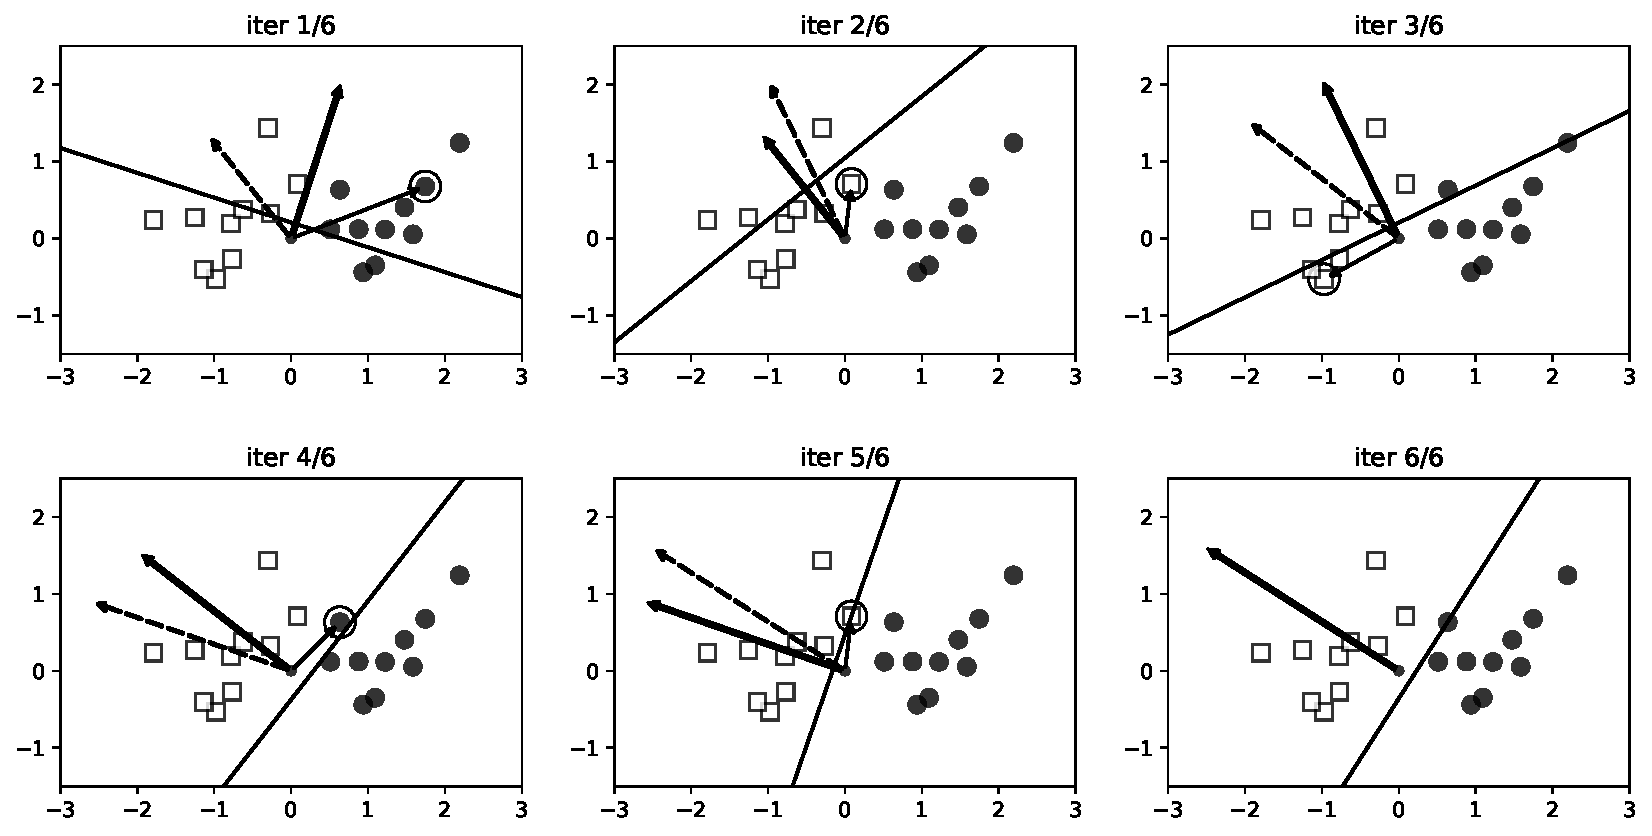
\includegraphics[width = \textwidth]{ebookML_src/src/perceptron/pla_visualize1.pdf}
\caption[]{Minh hoạ thuật toán perceptron. Các điểm hình vuông có nhãn bằng $1$, các điểm hình tròn có nhãn $-1$. Tại mỗi vòng lặp, đường thẳng là đường ranh giới. Vector pháp tuyến $\bw_t$ của đường thằng này là vector đậm nét liền. Điểm được khoanh tròn là một điểm bị phân loại lỗi $\bx_i$. Vector mảnh nét liền thể hiện vector $\bx_i$. Vector nét đứt thể hiện $\bw_{t+1}$. Nếu $y_i = 1$ (một điểm hình vuông), vector nét đứt bằng tổng hai vector kia. Nếu $y_i = -1$, vector nét đứt bằng hiệu hai vector kia.}
\label{fig:9_vis}
\end{figure}
% ******************************************************************************
% ******************************************************************************
\begin{figure}[h]
\begin{subfigure}{0.359\textwidth}
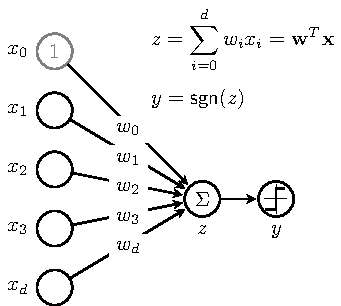
\includegraphics[width=1.02\linewidth]{Chapters/05_NeuralNetworks/09_perceptron/latex/pla_nn_a.pdf}
\caption{}
\label{fig:9_pla_lr_nna}
\end{subfigure}
\begin{subfigure}{0.3\textwidth}
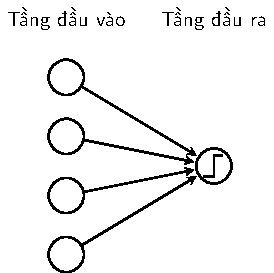
\includegraphics[width=1.02\linewidth]{Chapters/05_NeuralNetworks/09_perceptron/latex/pla_nn_b.pdf}
\caption{}
\label{fig:9_pla_lr_nnb}
\end{subfigure}
\begin{subfigure}{0.3\textwidth}
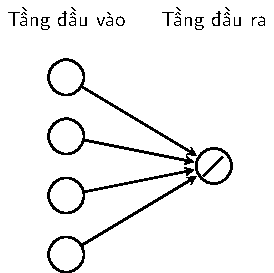
\includegraphics[width=1.02\linewidth]{Chapters/05_NeuralNetworks/09_perceptron/latex/lr_nn.pdf}
\caption{}
\label{fig:9_pla_lr_nnc}
\end{subfigure}
\caption{
Biểu diễn perceptron và hồi quy tuyến tính dưới dạng mạng neuron. (a) perceptron đầy đủ, (b) perceptron thu gọn, (c) hồi quy tuyến tính thu gọn.
}
\label{fig:9_pla_lr_nn}
\end{figure}
% ******************************************************************************

\section{Mô hình mạng neuron đầu tiên}
\index{mạng neuron -- neural network}
\index{neural network -- mạng neuron}
Hàm số dự đoán đầu ra của perceptron $\text{label}(\mathbf{x}) = \text{sgn}(\mathbf{w}^T\mathbf{x})$ được mô tả trên Hình~\ref{fig:9_pla_lr_nna}. Đây chính là dạng đơn giản nhất của một mạng neuron.

\index{tầng đầu vào -- input layer}
\index{input layer -- tầng đầu vào}
\index{hàm kích hoạt -- activation function}
\index{activation function -- hàm kích hoạt}
Đầu vào $\mathbf{x}$ của mạng được minh họa bằng các hình tròn bên trái gọi là
các \textit{nút}. Tập hợp các nút này được gọi là \textit{tầng đầu vào}. Số nút
trong tầng đầu vào là $d + 1$ với nút điều chỉnh $x_0$ đôi khi được ẩn đi và ngầm hiểu  bằng một. Các \textit{trọng số} $w_0, w_1, \dots, w_d$ được gán vào các mũi
tên đi tới nút $ z = \sum_{i=0}^dw_ix_i =
\bx^T\bw$. Nút $y = \text{sgn}(z)$ là đầu ra của
mạng. Ký hiệu hình chữ Z ngược trong nút $y$ thể hiện đồ thị của hàm
$\text{sgn}$. Hàm $y = \text{sgn}(z)$ đóng vai trò là một \textit{hàm kích
hoạt}. Có nhiều loại hàm kích hoạt khác nhau sẽ được trình bày trong các chương sau. Dữ liệu đầu vào được đặt tại tầng đầu vào, lấy tổng có trọng số lưu vào
biến $z$ rồi đi qua hàm kích hoạt để có kết quả ở $y$. Đây chính là dạng đơn
giản nhất của một mạng neuron nhân tạo. Perceptron cũng có thể được vẽ giản lược
như Hình~\ref{fig:9_pla_lr_nnb}, với ẩn ý rằng hàm tính tổng và hàm kích hoạt
được gộp làm một.

\index{tầng đầu ra -- output layer}
\index{output layer -- tầng đầu ra}
\index{tầng ẩn -- hidden layer}
\index{hidden layer -- tầng ẩn}
Các mạng neuron có thể có một hoặc nhiều nút ở đầu ra tạo thành một \textit{tầng
đầu ra}. Trong các mô hình phức tạp hơn, các mạng neuron có thể có thêm các tầng
trung gian giữa tầng đầu vào và tầng đầu ra gọi là \textit{tầng ẩn}. Chúng
ta sẽ đi sâu vào các mạng nhiều tầng ẩn ở Chương~\ref{cha:mlp}. Trước đó, chúng
ta sẽ tìm hiểu các mạng neuron đơn giản hơn không có tầng ẩn nào.

% . Trong đó node $x_0 = 1$ thường được ẩn đi. Node $z$ cũng được ẩn đi và viết gộp vào trong node $y$. Perceptron thường được vẽ dưới dạng đơn giản như Hình 5 bên phải.

Để ý rằng nếu thay hàm kích hoạt bởi hàm đồng nhất $y = z$, ta sẽ có một mạng neuron mô tả mô hình hồi quy tuyến tính như Hình~\ref{fig:9_pla_lr_nnc}.
Đường thẳng chéo trong nút đầu ra thể hiện đồ thị hàm số $y = z$. Các trục tọa độ đã
được lược bỏ.



\begin{figure}[t]
\centering
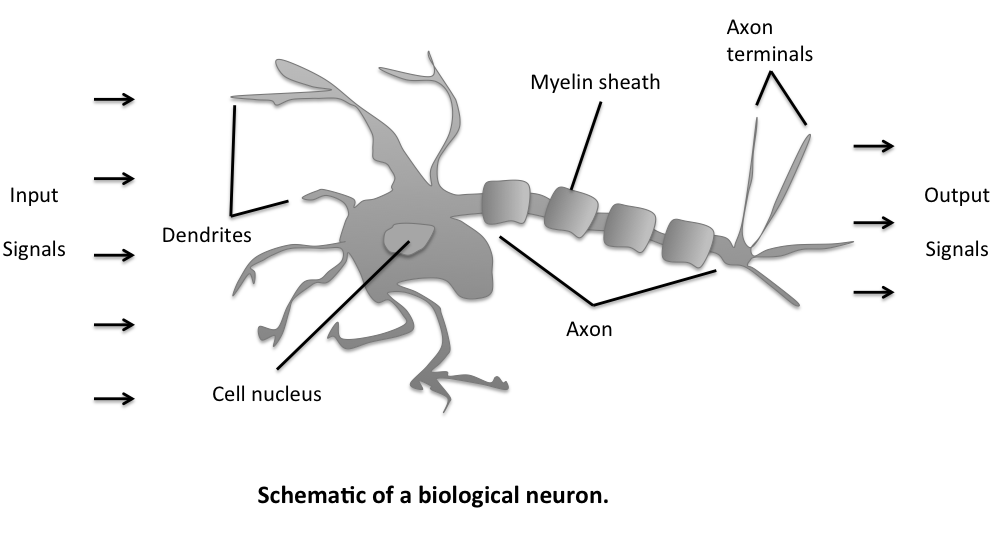
\includegraphics[width = \textwidth]{Chapters/05_NeuralNetworks/09_perceptron/perceptron_neuron_gray.png}
\caption{
Cấu trúc của một neuron thần kinh sinh học. Nguồn: \textit{Single-Layer Neural Networks and Gradient Descent} (\url{https://goo.gl/RjBREb}).
}
\label{fig:9_per_nn}
\end{figure}


% ******************************************************************************
% figure with side caption
% \begin{figure}[t]
%     % caption on side
%     \floatbox[{\capbeside\thisfloatsetup{capbesideposition={right,top},capbesidewidth=5cm}}]{figure}[\FBwidth]
%     {\caption{
%     Cấu trúc của một neuron thần kinh sinh học (Nguồn: \href{http://sebastianraschka.com/Articles/2015_singlelayer_neurons.html}{Single-Layer Neural Networks and Gradient Descent}).
%     }
%     \label{fig:9_per_nn}}
%     { % figure here
%     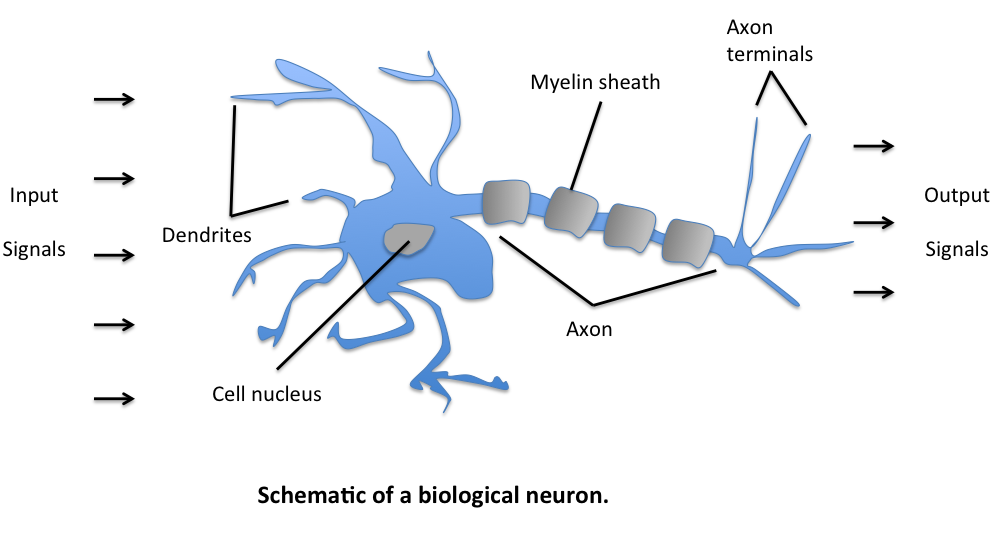
\includegraphics[width=.65\textwidth]{Chapters/05_NeuralNetworks/09_perceptron/perceptron_neuron.png}
%     }
% \end{figure}
% ******************************************************************************

% <div class="imgcap">
% <img src ="http://sebastianraschka.com/images/blog/2015/singlelayer_neural_networks_files/perceptron_neuron.png" align = "center" width = "600">
% <div class = "thecap">Hình 7: Mô tả một neuron thần kinh sinh học. (Nguồn: <a href = "http://sebastianraschka.com/Articles/2015_singlelayer_neurons.html">Single-Layer Neural Networks and Gradient Descent</a>)</div>
% </div>

% \begin{figure}[t]
%     % caption on side
%     \floatbox[{\capbeside\thisfloatsetup{capbesideposition={right,top},capbesidewidth=6cm}}]{figure}[\FBwidth]
%     {\caption{

%     }
%     \label{fig:}}
%     { % figure here
%     \includegraphics[width=.5\textwidth]{}
%     }
% \end{figure}

% {\color{red} IMG}


Mô hình perceptron ở trên khá giống với một thành phần nhỏ của mạng thần kinh
sinh học như Hình~\ref{fig:9_per_nn}. Dữ liệu từ nhiều dây thần kinh đầu vào đi
về một nhân tế bào. Nhân tế bào tổng hợp thông tin và đưa ra quyết định ở tín
hiệu đầu ra. Trong mạng neuron nhận tạo của perceptron, mỗi giá trị $x_i$ đóng
vai trò một tín hiệu đầu vào, hàm tính tổng và hàm kích hoạt có chức năng tương
tự nhân tế bào. Tên gọi \textit{mạng neuron nhân tạo} được khởi nguồn từ đây.

%  Thông tin được tổng hợp và được đưa ra ở output. Nhiều bộ phận như thế này kết hợp với nhau tạo nên hệ thần kinh sinh học. Chính vì vậy mà có tên Neural Networks trong Machine Learning. Đôi khi mạng này còn được gọi là Artificial Neural Networks (ANN) tức \textit{hệ neuron nhân tạo}.


\section{Thảo Luận}

\textit{PLA có thể cho vô số nghiệm khác nhau.}
Nếu hai tập dữ liệu tách biệt tuyến tính thì có vô số đường ranh giới như trong Hình~\ref{fig:9_6a}. Các đường khác nhau sẽ
quyết định điểm hình tam giác có nhãn khác nhau. Trong các đường đó, đường
nào là tốt nhất? Và định nghĩa ``tốt nhất'' được hiểu theo nghĩa nào? Các câu hỏi này sẽ được thảo luận kỹ hơn trong Chương~\ref{cha:svm}.


\textit{PLA đòi hỏi hai tập dữ liệu phải tách biệt tuyến tính}.
Hình~\ref{fig:9_6b} mô tả hai tập dữ liệu \textit{gần} tách biệt tuyến tính. Mỗi tập có một điểm {nhiễu} nằm lẫn tập còn lại. Trong trường hợp này, thuật toán PLA không bao giờ dừng lại vì luôn có ít nhất hai điểm bị phân loại lỗi.


%% *****************************************************************************
\begin{figure}[t]
\begin{subfigure}{0.49\textwidth}
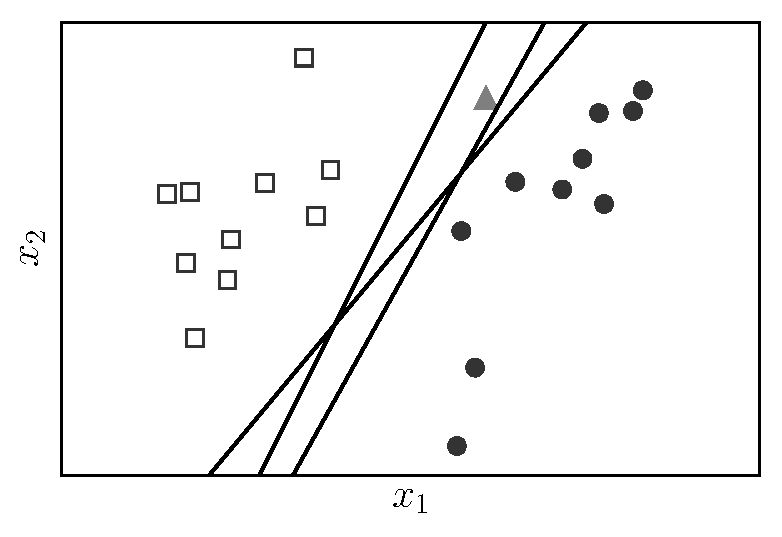
\includegraphics[width=0.99\linewidth]{ebookML_src/src/perceptron/pla6.pdf}
\caption{}
\label{fig:9_6a}
\end{subfigure}
\begin{subfigure}{0.49\textwidth}
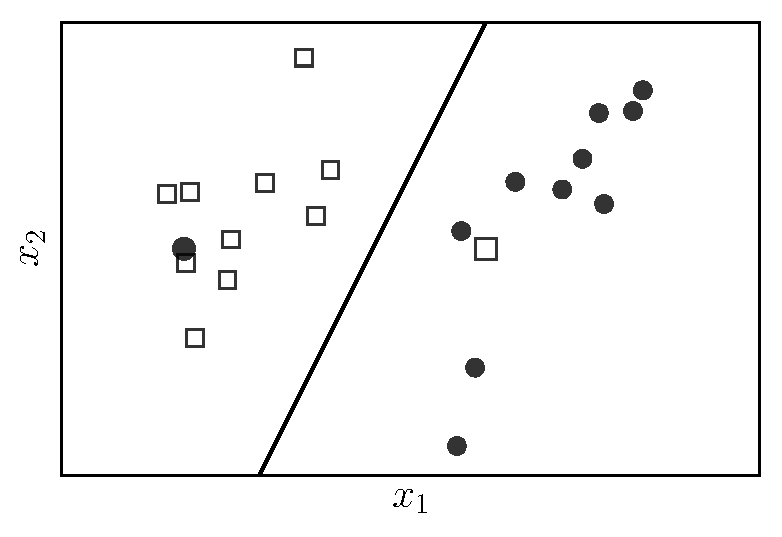
\includegraphics[width=0.99\linewidth]{ebookML_src/src/perceptron/pla7.pdf}
\caption{}
\label{fig:9_6b}
\end{subfigure}
\caption{
Với bài toán phân loại nhị phân, PLA có thể (a) cho vô số nghiệm, hoặc (b) vô nghiệm thậm chí khi có nhiễu nhỏ.
}
\label{fig:9_6}
\end{figure}
%% *****************************************************************************


Trong một chừng mực nào đó, đường thẳng màu đen vẫn có thể coi là một nghiệm tốt vì nó đã giúp phân loại chính xác hầu hết các điểm. Việc không hội tụ với dữ liệu \textit{gần} tách biệt tuyến tính là một nhược điểm lớn của PLA.

\index{thuật toán bỏ túi -- pocket algorithm}
\index{pocket algorithm -- thuật toán bỏ túi}
Nhược điểm này có thể được khắc phục bằng \textit{thuật toán bỏ túi} (\textit{pocket algorithm}).

\textit{Thuật toán bỏ túi}~\cite{abu2012learning}: một cách trực quan, nếu chỉ có
ít nhiễu, ta sẽ đi tìm một đường ranh giới sao cho có ít điểm bị phân loại lỗi
nhất. Việc này có thể được thực hiện thông qua PLA và thuật toán tìm số nhỏ nhất trong mảng một chiều:
\begin{itemize}
\item Giới hạn số lượng vòng lặp của PLA. Đặt nghiệm $\bw$ sau vòng lặp đầu tiên và số điểm bị phân loại lỗi vào trong \textit{túi}.

\item  Mỗi lần cập nhật nghiệm $\mathbf{w}_t$ mới, ta đếm xem có bao nhiêu điểm bị phân loại lỗi. So sánh số lượng này với số điểm bị phân loại lỗi trong túi. Nếu số lượng điểm bị phân loại lỗi này nhỏ hơn, tức ta đạt được mô hình tốt hơn trên tập huấn luyện, ta thay thế nghiệm trong túi bằng nghiệm mới và số điểm bị phân loại lỗi tương ứng. Lặp lại bước này đến khi hết số vòng lặp.
\end{itemize}



Mã nguồn trong chương này có thể được tìm thấy tại \url{https://goo.gl/tisSTq}.

% \section{Kết luận}

% Hy vọng rằng bài viết này sẽ giúp các bạn phần nào hiểu được một số khái niệm trong Neural Networks. Trong một số bài tiếp theo, tôi sẽ tiếp tục nói về các thuật toán cơ bản khác trong Neural Networks trước khi chuyển sang phần khác.

% Trong tương lai, nếu có thể, tôi sẽ viết tiếp về Deep Learning và chúng ta sẽ lại quay lại với Neural Networks.


% \section{Đ}

% [1] F. Rosenblatt. The perceptron, a perceiving and recognizing automaton Project Para. Cornell Aeronautical Laboratory, 1957.

% [2] W. S. McCulloch and W. Pitts. A logical calculus of the ideas immanent in nervous activity. The bulletin of mathematical biophysics, 5(4):115–133, 1943.

% [3] B. Widrow et al. Adaptive ``Adaline'' neuron using chemical ”memistors”. Number Technical Report 1553-2. Stanford Electron. Labs., Stanford, CA, October 1960.

% [3] Abu-Mostafa, Yaser S., Malik Magdon-Ismail, and Hsuan-Tien Lin. Learning from data. Vol. 4. New York, NY, USA:: AMLBook, 2012. (\href{http://work.caltech.edu/telecourse.html}{link to course})

% [4] Bishop, Christopher M. "Pattern recognition and Machine Learning.", Springer  (2006). (\href{http://users.isr.ist.utl.pt/~wurmd/Livros/school/Bishop%20-%20Pattern%20Recognition%20And%20Machine%20Learning%20-%20Springer%20%202006.pdf}{book})

% [5] Duda, Richard O., Peter E. Hart, and David G. Stork. Pattern classification. John Wiley \& Sons, 2012.
